% Keck DSST section

For a while, we believed that telluric contamination was the major culprit
behind the \keck\ RV-BC anomaly. However, the simulations in previous
section have revealed that tellurics probably only contribute a small
amount, mostly buried underneath photon noise and algorithmic
errors. We quickly focused our suspicion to DSST, because we saw the
differences in DSSTs before and after telluric cleaning (described in
Section~\ref{keck:telluric:real}), which are often larger than the
micro-telluric lines and could easily manifest as trends in the RV-BC
plane.

Any errors in the DSST, i.e., differences between the true stellar
spectrum and our assumed knowledge of truth (the DSST), are just like
persisting spectral contamination in the star's frame (instead of the
Earth's frame like the telluric contamination). Therefore, it beats
against the iodine lines as the stellar lines move back and forth
through the forest of iodine lines due to the Earth barycentric motion
and the star's intrinsic RV variation. As a result, it manifests as
anomalous RV-BC trends and adds bias and scatter to the final RVs.

We do know for sure that there are errors in the DSST, which could
arise from every step of its making. Here is an outline of how DSSTs
are made (also illustrated in Figure~\ref{keck:dsst:dsstmake}) with
highlights on potential sources of errors: 
\begin{enumerate}
\item A few high SNR, high resolution (using a narrower slit than
  the one for standard star$+$iodine frames) observations on the target
  stars are taken without the iodine cells. These are the bases for the
  DSST. The 1-D stellar spectra extracted from these frames are stacked
  together to raise the SNR, and {\em the stacking process could have errors
    from interpolation and rebinning}. Each chunk of the stacked 1-D
  stellar spectrum is also normalized before the final deconvolution,
  and {\em normalization errors can sneak in}.
\item Bracketing these stellar observations, both before and after,
  a couple of frames on nearby B star are taken through the iodine
  cell. These are the frames which anchor the wavelength solution
  and IPs for the stellar frames. The IPs derived from these frames
  are later used for deconvolving the stellar frames to make
  DSST. {\em The IPs in the B star $+$ iodine frames might be different from the
    ones in the stellar frames} because of, for example, changes in the
  telescope's PSF, changes in the spectrograph IPs due to the
  addition of the iodine cell in the light path, and so on. This
  could introduce errors in the DSST. {\em The wavelength solution of
    these two types of frames can also differ} for similar reasons, and
  although the wavelength zero point for each spectral chunk have a
  large tolerance for errors, {\em any errors in wavelength dispersion
  can translate into RV errors}.
\item Using the averaged IPs derived from the B star $+$ iodine
  frames, the stacked stellar spectrum is deconvolved. Its
  wavelength solution is determined by the averaged wavelength
  solution of the B star frames. Deconvolution is a ill-posed
  problem and does not have unique solutions, and therefore {\em errors
    in DSST can arise from the deconvolution algorithm employed}. 
\end{enumerate}

%----------------------------------------------------------------
% How DSST is made
% plot made by converting a slide in Berkeley-CIPS talk in 2015 talk
% tour into png the pdf then ps then eps 
\begin{figure}
\centering
\includegraphics[scale=0.42]{keck/dsstmake.eps}
\caption{Illustration of the making of DSST from deconvolution, using
  IPs derived from neighboring B star $+$ iodine observations.
\label{telluric:fig:dsstmake}}
\end{figure}
%----------------------------------------------------------------


However, the question is how much does a DSST differ from the real
stellar spectrum, and more importantly, how do these errors translate
into RV errors and how much. Is the RV-BC trend with $\sim$1~m/s
amplitude dominated by such errors?

To answer these questions, we performed simulations using synthetic
data and the Doppler code. In the previous section, when simulating
the effects of telluric lines, we used ``perfect DSSTs'' that are
simply the input synthetic stellar spectrum (no deconvolution
involved, of course), and naturally they do not have errors in them
(except for a small amount of interpolation errors). To study the
effects of errors in DSST, we need to bring back the deconvolution
process and simulate the entire process of the making of a DSST. In
the following texts, the true stellar spectrum, i.e., the synthetic
input stellar spectrum, is referred to as the ``true spectrum'', while
the DSST made based on simulated data is referred to as the
``simulated DSST'', as opposed to a real DSST which is derived from
real data.

Here is how we made a simulated DSST:
\begin{enumerate}
  \item Simulating the relevant observed data, using the same method
    as described in Section~\ref{keck:telluric:method}, which include:
    iodine-free stellar frames (normally 4--5 frames with high SNR) and a
    couple of B star $+$ iodine frames before and after the stellar
    frames. The B star $+$ iodine frames are simulated using the best-fit
    IPs and wavelength solutions derived from their real observation
    pairs. The IPs and wavelength solutions used in simulating the
    iodine-free stellar spectrum are from the same source. All of these
    simulated frames are free of telluric lines.
  \item Fitting the simulated B star $+$ iodine frames for wavelength
    solution and IPs, just as if they are real observed data.
  \item Using the fits on B star $+$ iodine frames to deconvolve the
    iodine-free stellar frames, and the result would be the simulated
    DSST. The codes used in this step are exactly the same ones in the
    CPS Doppler package.
\end{enumerate}

We then used the simulated DSST for RV extraction on an ensemble of
simulated star$+$iodine data (again, made in the same way as how we
made the telluric-free simulated data as described in
Section~\ref{keck:telluric:method}). We compare the RVs between the
extraction using the perfect DSST and the simulated DSST in
Figure~\ref{keck:fig:dsst}. Indeed, the errors in DSST are capable of
inducing RV-BC trends with an amplitude near 1~m/s. Because we used
the same IPs and wavelength solutions for the B star $+$ iodine frames
and the stellar frames, the errors in DSST we are probing here are
mostly from the deconvolution algorithm and random errors from the
photon noise and the CPS Doppler code/algorithm. The current CPS code
uses an unconventional ``deconvolution'' algorithm written by John
Johnson, which forward models the underlying stellar spectrum by
adding nodes of Gaussians at places of stellar lines, convolving that
with the derived IP from B star frames, and minimizing the $\chi^2$ to
find depths and positions of the Gaussian nodes. CPS has used other
deconvolution algorithms such as the Jansson constrained non-linear
method, which did not out-perform the current recipe using ``piston
Gaussians''.

The RV-BC patterns in the middle panels of Figure~\ref{keck:fig:dsst}
are different from the real observed RV-BC trends, which we
tentatively attribute to: (1) the synthetic spectrum is different from
the real stellar spectrum; (2) the noise and other random errors are
different, e.g., how IPs used in deconvolution can differ from the
real IPs due to the added photon noise, although they have the same
input in the simulation; (3) and the fact that there are other sources
of RV systematic errors in real data. Note that in reality, the
difference in IPs and wavelength solution between the B star and
stellar frames can rise from many more places besides photon noise.


%----------------------------------------------------------------
% Effect of imperfect DSST
% plot made by ~/Exo.../Keck.../simulate.../msplot.pro, plot_name='3panel'
\begin{figure}
\subfloat[HD 185144]{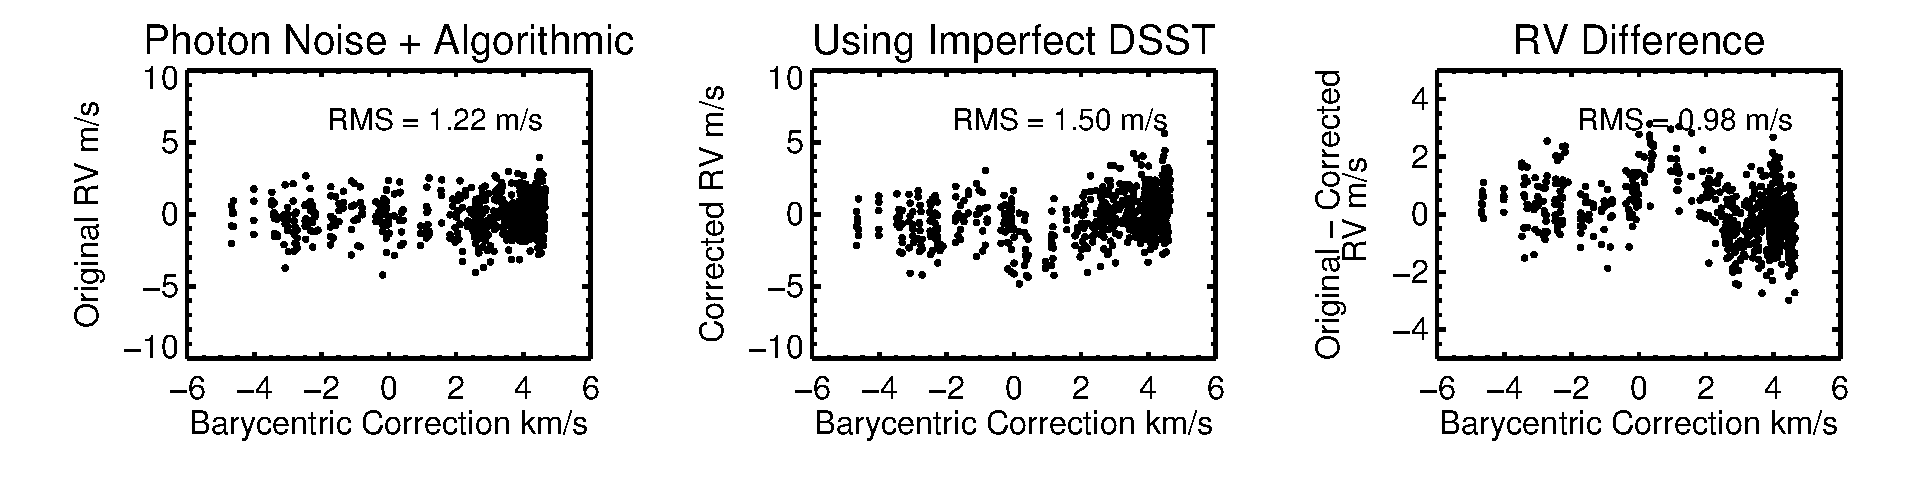
\includegraphics[scale=0.42]{keck/185144-rv-bc-3panel-test0-testd0.eps}}\
\subfloat[HD 10700]{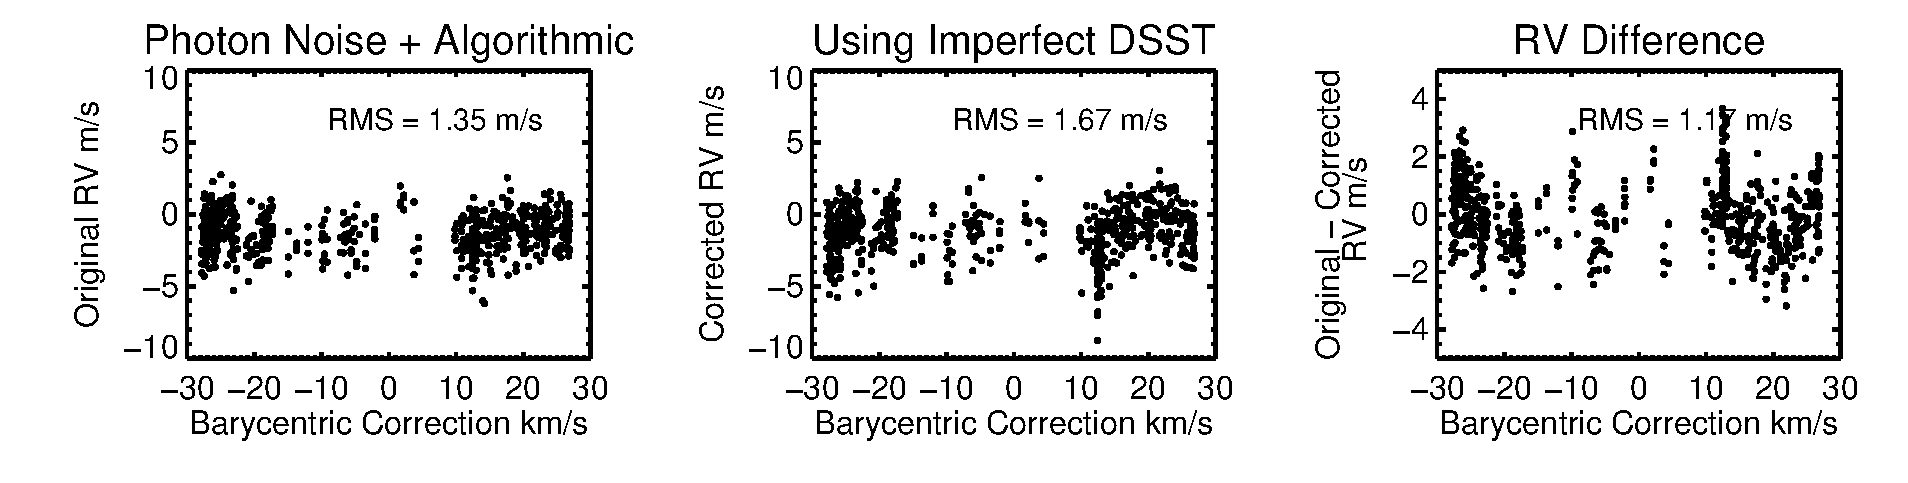
\includegraphics[scale=0.42]{keck/10700-rv-bc-3panel-test0-testd0.eps}}\
\caption{Effect of imperfect DSST as revealed by simulated data. The top
  panels are for HD 185144 and the bottom panels are for HD 10700. The
  left panels are RVs from the simulation run using the perfect DSST
  or the true spectrum. The middle panels are RVs from the simulation
  run using the simulated DSST, which has errors from the manufacture
  process of DSST such as the deconvolution. The right panels are RV
  differences between the left and the middle ones, illustrating the
  effects of DSST errors on RV precision and accuracy, because the
  only difference between these two runs is the DSST.
\label{keck:fig:dsst}}
\end{figure}
%----------------------------------------------------------------


We then compared the simulated DSST to the true spectrum (the input
synthetic spectrum), which revealed small but non-negligible
differences, as illustrated in the left panels of
Figure~\ref{keck:fig:dsstchunk}. The effects on RVs rising from these
differences are also illustrated in Figure~\ref{keck:fig:dsstchunk},
in the right panels. These are cherry-picked chunks which show the
same RV-BC patterns in simulation and real observations. Why some
chunks are as such but others show different patterns between
simulation and reality? The answer to this question will shine some
light on the original of the DSST errors and hopefully even a remedy,
which will be one of the focuses of future works. We summarize our
conclusion and lay out future works in the final section of this chapter.


%----------------------------------------------------------------
% Chunk illustration of effect of imperfect DSST
% plot made by ~/Exo.../Keck.../simulate.../msplot.pro, plot_name='makefakedsst','chunkcomp'
\begin{figure}
\subfloat{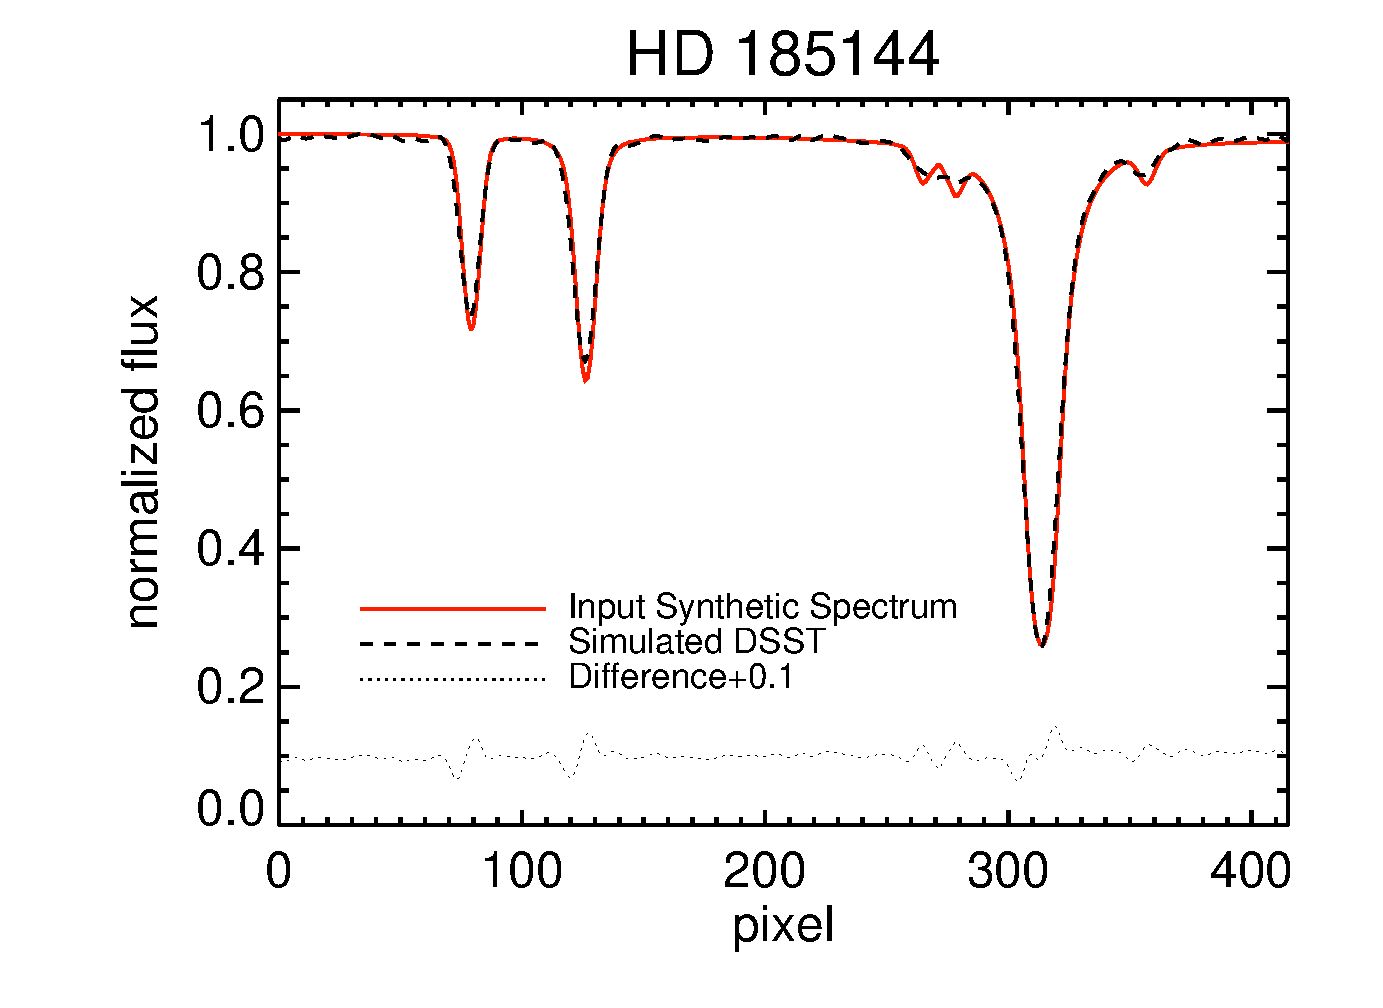
\includegraphics[scale=0.3]{keck/185144_makefakedsst_100.eps}}
\subfloat{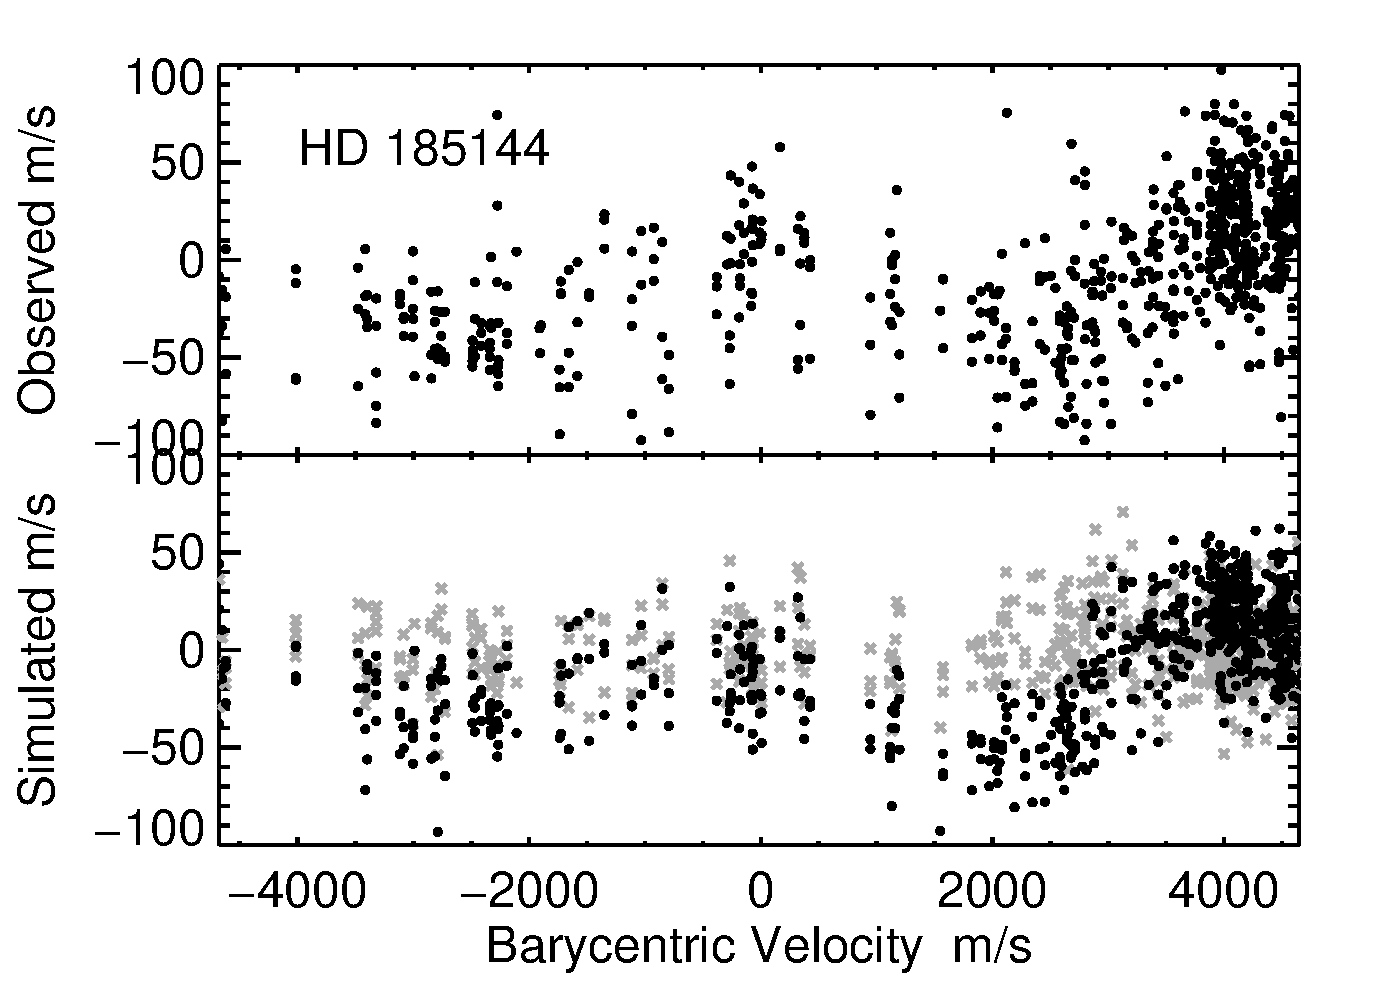
\includegraphics[scale=0.3]{keck/185144_chunkcomp_100.eps}}\
\subfloat{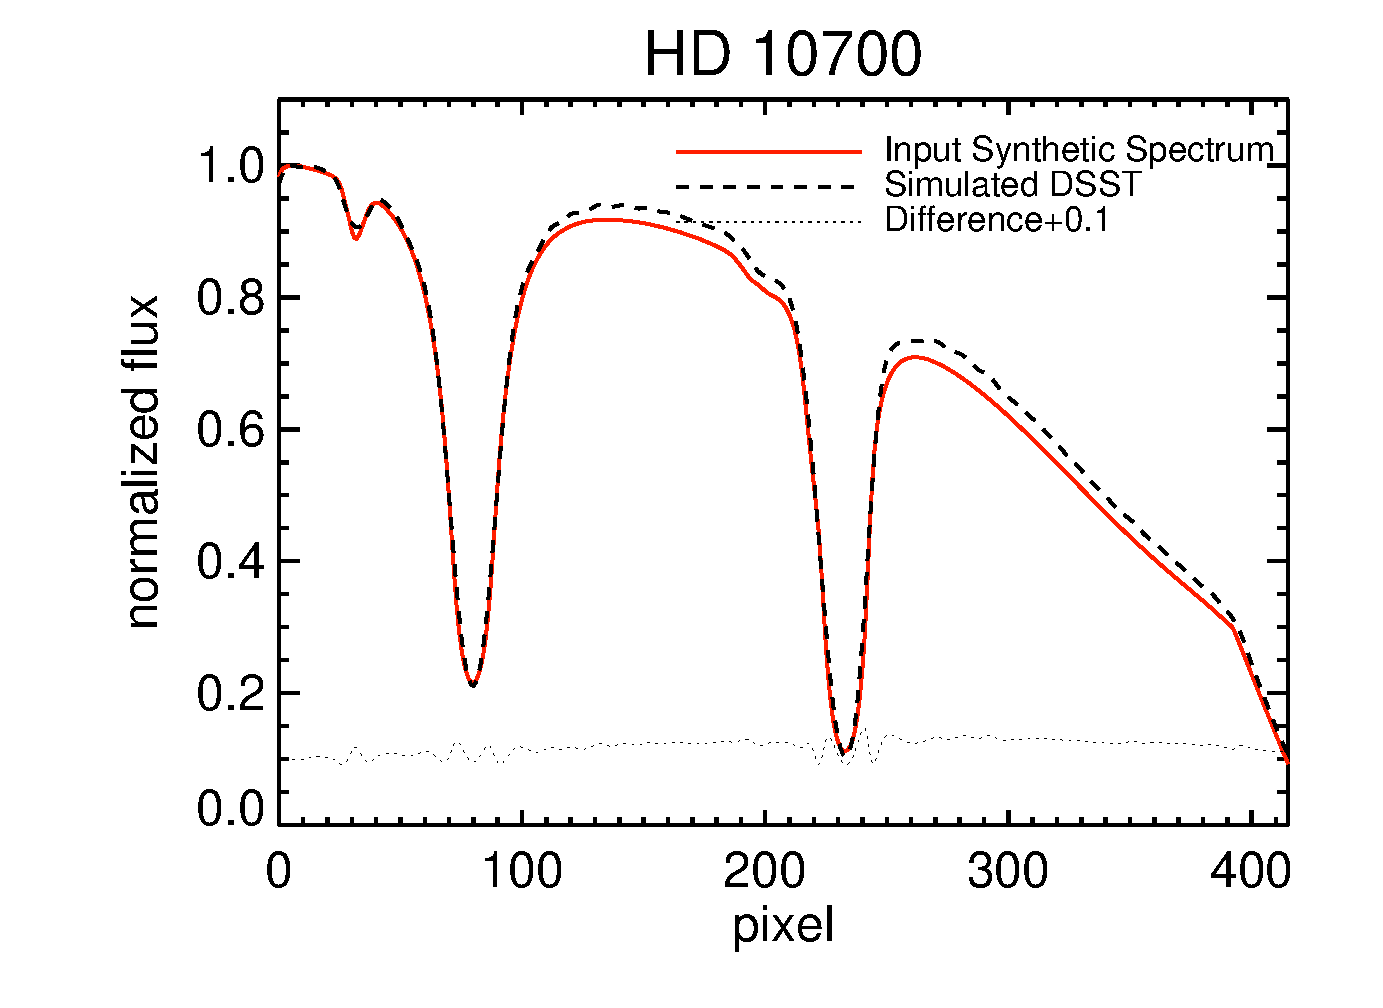
\includegraphics[scale=0.3]{keck/10700_makefakedsst_104.eps}}
\subfloat{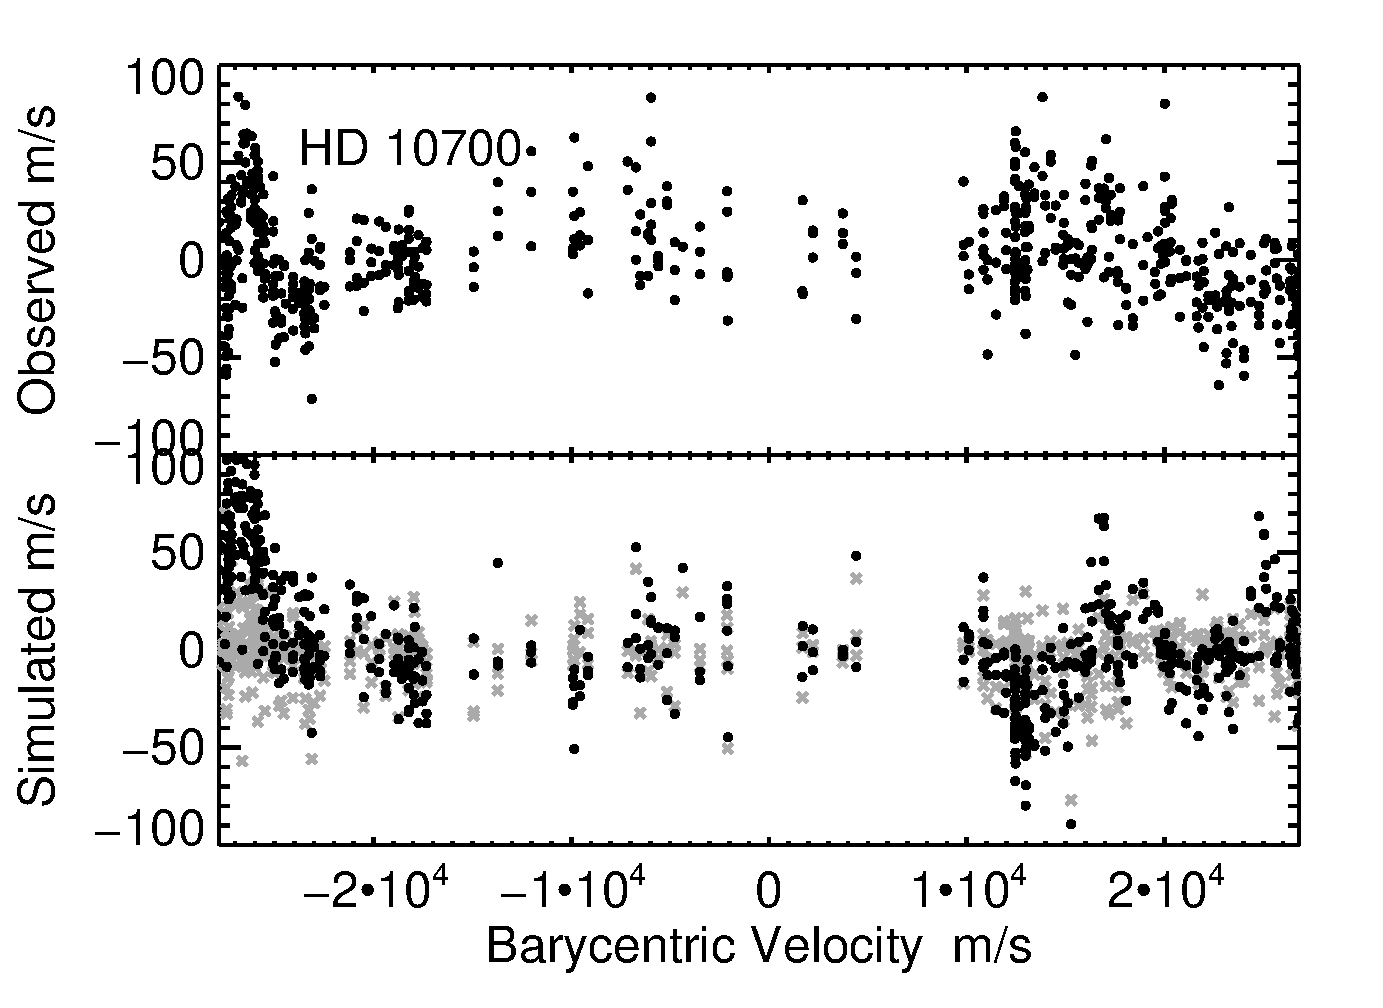
\includegraphics[scale=0.3]{keck/10700_chunkcomp_104.eps}}\
\caption{Effect of imperfect DSST on simulated data for a single
spectral chunk. The top panels are for a chunk near 5160\AA\ for HD
185144, and the bottom panels are for a chunk around 5166\AA\ for HD
10700. The left panels illustrate the differences between the
simulated DSST (solid red) and the true spectrum (dashed black), i.e.,
the errors in DSST. The right panels show the derived RVs for this
chunk as a function of BC: the RVs on top, with $y$-axis labeled as
``Observed'', are from real \keck\ data, and RVs below, labeled with
``Simulated'', are from simulations using the simulated DSST (black
dots) and the ``perfect'' simulation using the true spectrum as the
DSST (gray dots, with no apparent RV-BC trends). The $\sim$
5100--5200\AA\ spectral region tends to receive high weights due to
its high density of stellar and iodine lines and a lack of telluric
lines.
\label{keck:fig:dsstchunk}}
\end{figure}
%----------------------------------------------------------------
